\documentclass{article} % For LaTeX2e
% Compile with XeLaTeX (Vietnamese text):  xelatex Group06_ProgressReport.tex  (run twice)
\usepackage{iclr2027_conference}
\usepackage{fontspec}
\setmainfont{texgyretermes}[Extension=.otf, UprightFont=*-regular, BoldFont=*-bold, ItalicFont=*-italic, BoldItalicFont=*-bolditalic]

% Optional math commands from https://github.com/goodfeli/dlbook_notation.
%%%%% NEW MATH DEFINITIONS %%%%%

\usepackage{amsmath,amsfonts,bm}

% Mark sections of captions for referring to divisions of figures
\newcommand{\figleft}{{\em (Left)}}
\newcommand{\figcenter}{{\em (Center)}}
\newcommand{\figright}{{\em (Right)}}
\newcommand{\figtop}{{\em (Top)}}
\newcommand{\figbottom}{{\em (Bottom)}}
\newcommand{\captiona}{{\em (a)}}
\newcommand{\captionb}{{\em (b)}}
\newcommand{\captionc}{{\em (c)}}
\newcommand{\captiond}{{\em (d)}}

% Highlight a newly defined term
\newcommand{\newterm}[1]{{\bf #1}}


% Figure reference, lower-case.
\def\figref#1{figure~\ref{#1}}
% Figure reference, capital. For start of sentence
\def\Figref#1{Figure~\ref{#1}}
\def\twofigref#1#2{figures \ref{#1} and \ref{#2}}
\def\quadfigref#1#2#3#4{figures \ref{#1}, \ref{#2}, \ref{#3} and \ref{#4}}
% Section reference, lower-case.
\def\secref#1{section~\ref{#1}}
% Section reference, capital.
\def\Secref#1{Section~\ref{#1}}
% Reference to two sections.
\def\twosecrefs#1#2{sections \ref{#1} and \ref{#2}}
% Reference to three sections.
\def\secrefs#1#2#3{sections \ref{#1}, \ref{#2} and \ref{#3}}
% Reference to an equation, lower-case.
\def\eqref#1{equation~\ref{#1}}
% Reference to an equation, upper case
\def\Eqref#1{Equation~\ref{#1}}
% A raw reference to an equation---avoid using if possible
\def\plaineqref#1{\ref{#1}}
% Reference to a chapter, lower-case.
\def\chapref#1{chapter~\ref{#1}}
% Reference to an equation, upper case.
\def\Chapref#1{Chapter~\ref{#1}}
% Reference to a range of chapters
\def\rangechapref#1#2{chapters\ref{#1}--\ref{#2}}
% Reference to an algorithm, lower-case.
\def\algref#1{algorithm~\ref{#1}}
% Reference to an algorithm, upper case.
\def\Algref#1{Algorithm~\ref{#1}}
\def\twoalgref#1#2{algorithms \ref{#1} and \ref{#2}}
\def\Twoalgref#1#2{Algorithms \ref{#1} and \ref{#2}}
% Reference to a part, lower case
\def\partref#1{part~\ref{#1}}
% Reference to a part, upper case
\def\Partref#1{Part~\ref{#1}}
\def\twopartref#1#2{parts \ref{#1} and \ref{#2}}

\def\ceil#1{\lceil #1 \rceil}
\def\floor#1{\lfloor #1 \rfloor}
\def\1{\bm{1}}
\newcommand{\train}{\mathcal{D}}
\newcommand{\valid}{\mathcal{D_{\mathrm{valid}}}}
\newcommand{\test}{\mathcal{D_{\mathrm{test}}}}

\def\eps{{\epsilon}}


% Random variables
\def\reta{{\textnormal{$\eta$}}}
\def\ra{{\textnormal{a}}}
\def\rb{{\textnormal{b}}}
\def\rc{{\textnormal{c}}}
\def\rd{{\textnormal{d}}}
\def\re{{\textnormal{e}}}
\def\rf{{\textnormal{f}}}
\def\rg{{\textnormal{g}}}
\def\rh{{\textnormal{h}}}
\def\ri{{\textnormal{i}}}
\def\rj{{\textnormal{j}}}
\def\rk{{\textnormal{k}}}
\def\rl{{\textnormal{l}}}
% rm is already a command, just don't name any random variables m
\def\rn{{\textnormal{n}}}
\def\ro{{\textnormal{o}}}
\def\rp{{\textnormal{p}}}
\def\rq{{\textnormal{q}}}
\def\rr{{\textnormal{r}}}
\def\rs{{\textnormal{s}}}
\def\rt{{\textnormal{t}}}
\def\ru{{\textnormal{u}}}
\def\rv{{\textnormal{v}}}
\def\rw{{\textnormal{w}}}
\def\rx{{\textnormal{x}}}
\def\ry{{\textnormal{y}}}
\def\rz{{\textnormal{z}}}

% Random vectors
\def\rvepsilon{{\mathbf{\epsilon}}}
\def\rvtheta{{\mathbf{\theta}}}
\def\rva{{\mathbf{a}}}
\def\rvb{{\mathbf{b}}}
\def\rvc{{\mathbf{c}}}
\def\rvd{{\mathbf{d}}}
\def\rve{{\mathbf{e}}}
\def\rvf{{\mathbf{f}}}
\def\rvg{{\mathbf{g}}}
\def\rvh{{\mathbf{h}}}
\def\rvu{{\mathbf{i}}}
\def\rvj{{\mathbf{j}}}
\def\rvk{{\mathbf{k}}}
\def\rvl{{\mathbf{l}}}
\def\rvm{{\mathbf{m}}}
\def\rvn{{\mathbf{n}}}
\def\rvo{{\mathbf{o}}}
\def\rvp{{\mathbf{p}}}
\def\rvq{{\mathbf{q}}}
\def\rvr{{\mathbf{r}}}
\def\rvs{{\mathbf{s}}}
\def\rvt{{\mathbf{t}}}
\def\rvu{{\mathbf{u}}}
\def\rvv{{\mathbf{v}}}
\def\rvw{{\mathbf{w}}}
\def\rvx{{\mathbf{x}}}
\def\rvy{{\mathbf{y}}}
\def\rvz{{\mathbf{z}}}

% Elements of random vectors
\def\erva{{\textnormal{a}}}
\def\ervb{{\textnormal{b}}}
\def\ervc{{\textnormal{c}}}
\def\ervd{{\textnormal{d}}}
\def\erve{{\textnormal{e}}}
\def\ervf{{\textnormal{f}}}
\def\ervg{{\textnormal{g}}}
\def\ervh{{\textnormal{h}}}
\def\ervi{{\textnormal{i}}}
\def\ervj{{\textnormal{j}}}
\def\ervk{{\textnormal{k}}}
\def\ervl{{\textnormal{l}}}
\def\ervm{{\textnormal{m}}}
\def\ervn{{\textnormal{n}}}
\def\ervo{{\textnormal{o}}}
\def\ervp{{\textnormal{p}}}
\def\ervq{{\textnormal{q}}}
\def\ervr{{\textnormal{r}}}
\def\ervs{{\textnormal{s}}}
\def\ervt{{\textnormal{t}}}
\def\ervu{{\textnormal{u}}}
\def\ervv{{\textnormal{v}}}
\def\ervw{{\textnormal{w}}}
\def\ervx{{\textnormal{x}}}
\def\ervy{{\textnormal{y}}}
\def\ervz{{\textnormal{z}}}

% Random matrices
\def\rmA{{\mathbf{A}}}
\def\rmB{{\mathbf{B}}}
\def\rmC{{\mathbf{C}}}
\def\rmD{{\mathbf{D}}}
\def\rmE{{\mathbf{E}}}
\def\rmF{{\mathbf{F}}}
\def\rmG{{\mathbf{G}}}
\def\rmH{{\mathbf{H}}}
\def\rmI{{\mathbf{I}}}
\def\rmJ{{\mathbf{J}}}
\def\rmK{{\mathbf{K}}}
\def\rmL{{\mathbf{L}}}
\def\rmM{{\mathbf{M}}}
\def\rmN{{\mathbf{N}}}
\def\rmO{{\mathbf{O}}}
\def\rmP{{\mathbf{P}}}
\def\rmQ{{\mathbf{Q}}}
\def\rmR{{\mathbf{R}}}
\def\rmS{{\mathbf{S}}}
\def\rmT{{\mathbf{T}}}
\def\rmU{{\mathbf{U}}}
\def\rmV{{\mathbf{V}}}
\def\rmW{{\mathbf{W}}}
\def\rmX{{\mathbf{X}}}
\def\rmY{{\mathbf{Y}}}
\def\rmZ{{\mathbf{Z}}}

% Elements of random matrices
\def\ermA{{\textnormal{A}}}
\def\ermB{{\textnormal{B}}}
\def\ermC{{\textnormal{C}}}
\def\ermD{{\textnormal{D}}}
\def\ermE{{\textnormal{E}}}
\def\ermF{{\textnormal{F}}}
\def\ermG{{\textnormal{G}}}
\def\ermH{{\textnormal{H}}}
\def\ermI{{\textnormal{I}}}
\def\ermJ{{\textnormal{J}}}
\def\ermK{{\textnormal{K}}}
\def\ermL{{\textnormal{L}}}
\def\ermM{{\textnormal{M}}}
\def\ermN{{\textnormal{N}}}
\def\ermO{{\textnormal{O}}}
\def\ermP{{\textnormal{P}}}
\def\ermQ{{\textnormal{Q}}}
\def\ermR{{\textnormal{R}}}
\def\ermS{{\textnormal{S}}}
\def\ermT{{\textnormal{T}}}
\def\ermU{{\textnormal{U}}}
\def\ermV{{\textnormal{V}}}
\def\ermW{{\textnormal{W}}}
\def\ermX{{\textnormal{X}}}
\def\ermY{{\textnormal{Y}}}
\def\ermZ{{\textnormal{Z}}}

% Vectors
\def\vzero{{\bm{0}}}
\def\vone{{\bm{1}}}
\def\vmu{{\bm{\mu}}}
\def\vtheta{{\bm{\theta}}}
\def\va{{\bm{a}}}
\def\vb{{\bm{b}}}
\def\vc{{\bm{c}}}
\def\vd{{\bm{d}}}
\def\ve{{\bm{e}}}
\def\vf{{\bm{f}}}
\def\vg{{\bm{g}}}
\def\vh{{\bm{h}}}
\def\vi{{\bm{i}}}
\def\vj{{\bm{j}}}
\def\vk{{\bm{k}}}
\def\vl{{\bm{l}}}
\def\vm{{\bm{m}}}
\def\vn{{\bm{n}}}
\def\vo{{\bm{o}}}
\def\vp{{\bm{p}}}
\def\vq{{\bm{q}}}
\def\vr{{\bm{r}}}
\def\vs{{\bm{s}}}
\def\vt{{\bm{t}}}
\def\vu{{\bm{u}}}
\def\vv{{\bm{v}}}
\def\vw{{\bm{w}}}
\def\vx{{\bm{x}}}
\def\vy{{\bm{y}}}
\def\vz{{\bm{z}}}

% Elements of vectors
\def\evalpha{{\alpha}}
\def\evbeta{{\beta}}
\def\evepsilon{{\epsilon}}
\def\evlambda{{\lambda}}
\def\evomega{{\omega}}
\def\evmu{{\mu}}
\def\evpsi{{\psi}}
\def\evsigma{{\sigma}}
\def\evtheta{{\theta}}
\def\eva{{a}}
\def\evb{{b}}
\def\evc{{c}}
\def\evd{{d}}
\def\eve{{e}}
\def\evf{{f}}
\def\evg{{g}}
\def\evh{{h}}
\def\evi{{i}}
\def\evj{{j}}
\def\evk{{k}}
\def\evl{{l}}
\def\evm{{m}}
\def\evn{{n}}
\def\evo{{o}}
\def\evp{{p}}
\def\evq{{q}}
\def\evr{{r}}
\def\evs{{s}}
\def\evt{{t}}
\def\evu{{u}}
\def\evv{{v}}
\def\evw{{w}}
\def\evx{{x}}
\def\evy{{y}}
\def\evz{{z}}

% Matrix
\def\mA{{\bm{A}}}
\def\mB{{\bm{B}}}
\def\mC{{\bm{C}}}
\def\mD{{\bm{D}}}
\def\mE{{\bm{E}}}
\def\mF{{\bm{F}}}
\def\mG{{\bm{G}}}
\def\mH{{\bm{H}}}
\def\mI{{\bm{I}}}
\def\mJ{{\bm{J}}}
\def\mK{{\bm{K}}}
\def\mL{{\bm{L}}}
\def\mM{{\bm{M}}}
\def\mN{{\bm{N}}}
\def\mO{{\bm{O}}}
\def\mP{{\bm{P}}}
\def\mQ{{\bm{Q}}}
\def\mR{{\bm{R}}}
\def\mS{{\bm{S}}}
\def\mT{{\bm{T}}}
\def\mU{{\bm{U}}}
\def\mV{{\bm{V}}}
\def\mW{{\bm{W}}}
\def\mX{{\bm{X}}}
\def\mY{{\bm{Y}}}
\def\mZ{{\bm{Z}}}
\def\mBeta{{\bm{\beta}}}
\def\mPhi{{\bm{\Phi}}}
\def\mLambda{{\bm{\Lambda}}}
\def\mSigma{{\bm{\Sigma}}}

% Tensor
\DeclareMathAlphabet{\mathsfit}{\encodingdefault}{\sfdefault}{m}{sl}
\SetMathAlphabet{\mathsfit}{bold}{\encodingdefault}{\sfdefault}{bx}{n}
\newcommand{\tens}[1]{\bm{\mathsfit{#1}}}
\def\tA{{\tens{A}}}
\def\tB{{\tens{B}}}
\def\tC{{\tens{C}}}
\def\tD{{\tens{D}}}
\def\tE{{\tens{E}}}
\def\tF{{\tens{F}}}
\def\tG{{\tens{G}}}
\def\tH{{\tens{H}}}
\def\tI{{\tens{I}}}
\def\tJ{{\tens{J}}}
\def\tK{{\tens{K}}}
\def\tL{{\tens{L}}}
\def\tM{{\tens{M}}}
\def\tN{{\tens{N}}}
\def\tO{{\tens{O}}}
\def\tP{{\tens{P}}}
\def\tQ{{\tens{Q}}}
\def\tR{{\tens{R}}}
\def\tS{{\tens{S}}}
\def\tT{{\tens{T}}}
\def\tU{{\tens{U}}}
\def\tV{{\tens{V}}}
\def\tW{{\tens{W}}}
\def\tX{{\tens{X}}}
\def\tY{{\tens{Y}}}
\def\tZ{{\tens{Z}}}


% Graph
\def\gA{{\mathcal{A}}}
\def\gB{{\mathcal{B}}}
\def\gC{{\mathcal{C}}}
\def\gD{{\mathcal{D}}}
\def\gE{{\mathcal{E}}}
\def\gF{{\mathcal{F}}}
\def\gG{{\mathcal{G}}}
\def\gH{{\mathcal{H}}}
\def\gI{{\mathcal{I}}}
\def\gJ{{\mathcal{J}}}
\def\gK{{\mathcal{K}}}
\def\gL{{\mathcal{L}}}
\def\gM{{\mathcal{M}}}
\def\gN{{\mathcal{N}}}
\def\gO{{\mathcal{O}}}
\def\gP{{\mathcal{P}}}
\def\gQ{{\mathcal{Q}}}
\def\gR{{\mathcal{R}}}
\def\gS{{\mathcal{S}}}
\def\gT{{\mathcal{T}}}
\def\gU{{\mathcal{U}}}
\def\gV{{\mathcal{V}}}
\def\gW{{\mathcal{W}}}
\def\gX{{\mathcal{X}}}
\def\gY{{\mathcal{Y}}}
\def\gZ{{\mathcal{Z}}}

% Sets
\def\sA{{\mathbb{A}}}
\def\sB{{\mathbb{B}}}
\def\sC{{\mathbb{C}}}
\def\sD{{\mathbb{D}}}
% Don't use a set called E, because this would be the same as our symbol
% for expectation.
\def\sF{{\mathbb{F}}}
\def\sG{{\mathbb{G}}}
\def\sH{{\mathbb{H}}}
\def\sI{{\mathbb{I}}}
\def\sJ{{\mathbb{J}}}
\def\sK{{\mathbb{K}}}
\def\sL{{\mathbb{L}}}
\def\sM{{\mathbb{M}}}
\def\sN{{\mathbb{N}}}
\def\sO{{\mathbb{O}}}
\def\sP{{\mathbb{P}}}
\def\sQ{{\mathbb{Q}}}
\def\sR{{\mathbb{R}}}
\def\sS{{\mathbb{S}}}
\def\sT{{\mathbb{T}}}
\def\sU{{\mathbb{U}}}
\def\sV{{\mathbb{V}}}
\def\sW{{\mathbb{W}}}
\def\sX{{\mathbb{X}}}
\def\sY{{\mathbb{Y}}}
\def\sZ{{\mathbb{Z}}}

% Entries of a matrix
\def\emLambda{{\Lambda}}
\def\emA{{A}}
\def\emB{{B}}
\def\emC{{C}}
\def\emD{{D}}
\def\emE{{E}}
\def\emF{{F}}
\def\emG{{G}}
\def\emH{{H}}
\def\emI{{I}}
\def\emJ{{J}}
\def\emK{{K}}
\def\emL{{L}}
\def\emM{{M}}
\def\emN{{N}}
\def\emO{{O}}
\def\emP{{P}}
\def\emQ{{Q}}
\def\emR{{R}}
\def\emS{{S}}
\def\emT{{T}}
\def\emU{{U}}
\def\emV{{V}}
\def\emW{{W}}
\def\emX{{X}}
\def\emY{{Y}}
\def\emZ{{Z}}
\def\emSigma{{\Sigma}}

% entries of a tensor
% Same font as tensor, without \bm wrapper
\newcommand{\etens}[1]{\mathsfit{#1}}
\def\etLambda{{\etens{\Lambda}}}
\def\etA{{\etens{A}}}
\def\etB{{\etens{B}}}
\def\etC{{\etens{C}}}
\def\etD{{\etens{D}}}
\def\etE{{\etens{E}}}
\def\etF{{\etens{F}}}
\def\etG{{\etens{G}}}
\def\etH{{\etens{H}}}
\def\etI{{\etens{I}}}
\def\etJ{{\etens{J}}}
\def\etK{{\etens{K}}}
\def\etL{{\etens{L}}}
\def\etM{{\etens{M}}}
\def\etN{{\etens{N}}}
\def\etO{{\etens{O}}}
\def\etP{{\etens{P}}}
\def\etQ{{\etens{Q}}}
\def\etR{{\etens{R}}}
\def\etS{{\etens{S}}}
\def\etT{{\etens{T}}}
\def\etU{{\etens{U}}}
\def\etV{{\etens{V}}}
\def\etW{{\etens{W}}}
\def\etX{{\etens{X}}}
\def\etY{{\etens{Y}}}
\def\etZ{{\etens{Z}}}

% The true underlying data generating distribution
\newcommand{\pdata}{p_{\rm{data}}}
% The empirical distribution defined by the training set
\newcommand{\ptrain}{\hat{p}_{\rm{data}}}
\newcommand{\Ptrain}{\hat{P}_{\rm{data}}}
% The model distribution
\newcommand{\pmodel}{p_{\rm{model}}}
\newcommand{\Pmodel}{P_{\rm{model}}}
\newcommand{\ptildemodel}{\tilde{p}_{\rm{model}}}
% Stochastic autoencoder distributions
\newcommand{\pencode}{p_{\rm{encoder}}}
\newcommand{\pdecode}{p_{\rm{decoder}}}
\newcommand{\precons}{p_{\rm{reconstruct}}}

\newcommand{\laplace}{\mathrm{Laplace}} % Laplace distribution

\newcommand{\E}{\mathbb{E}}
\newcommand{\Ls}{\mathcal{L}}
\newcommand{\R}{\mathbb{R}}
\newcommand{\emp}{\tilde{p}}
\newcommand{\lr}{\alpha}
\newcommand{\reg}{\lambda}
\newcommand{\rect}{\mathrm{rectifier}}
\newcommand{\softmax}{\mathrm{softmax}}
\newcommand{\sigmoid}{\sigma}
\newcommand{\softplus}{\zeta}
\newcommand{\KL}{D_{\mathrm{KL}}}
\newcommand{\Var}{\mathrm{Var}}
\newcommand{\standarderror}{\mathrm{SE}}
\newcommand{\Cov}{\mathrm{Cov}}
% Wolfram Mathworld says $L^2$ is for function spaces and $\ell^2$ is for vectors
% But then they seem to use $L^2$ for vectors throughout the site, and so does
% wikipedia.
\newcommand{\normlzero}{L^0}
\newcommand{\normlone}{L^1}
\newcommand{\normltwo}{L^2}
\newcommand{\normlp}{L^p}
\newcommand{\normmax}{L^\infty}

\newcommand{\parents}{Pa} % See usage in notation.tex. Chosen to match Daphne's book.

\DeclareMathOperator*{\argmax}{arg\,max}
\DeclareMathOperator*{\argmin}{arg\,min}

\DeclareMathOperator{\sign}{sign}
\DeclareMathOperator{\Tr}{Tr}
\let\ab\allowbreak


\usepackage{hyperref}
\usepackage{url}
\usepackage{booktabs}
\usepackage{graphicx}
\usepackage{xcolor}
\usepackage{enumitem}
\usepackage{float}
\usepackage{wrapfig}
\setlist{nosep, leftmargin=1.1em}
\setlength{\textfloatsep}{7pt plus 2pt minus 2pt}
\setlength{\intextsep}{6pt plus 2pt minus 2pt}
\setlength{\abovecaptionskip}{3pt}
\setlength{\belowcaptionskip}{2pt}
\usepackage{tikz}
\usetikzlibrary{arrows.meta,positioning,calc}
\usepackage{pgfplots}
\pgfplotsset{compat=1.18}
\definecolor{cblue}{HTML}{1F5F8B}
\definecolor{cred}{HTML}{9B2C2C}
\definecolor{cgreen}{HTML}{2F7D4F}
\definecolor{camber}{HTML}{B7791F}
\definecolor{cgray}{HTML}{A0A7B2}
\pgfplotsset{lexstyle/.style={
  font=\scriptsize, tick label style={font=\scriptsize}, label style={font=\scriptsize},
  legend style={font=\scriptsize, draw=none, fill=none},
  axis line style={black!60}, tick style={black!60}, major grid style={black!12}, tick pos=left}}

% ---------------------------------------------------------------- results (filled from run finetune_v1_20261123)
% generated by scripts/make_report_results.py -- do not edit by hand
\newcommand{\ResZsMrr}{0.539}
\newcommand{\ResZsRten}{0.742}
\newcommand{\ResZsCeMrr}{0.624}
\newcommand{\ResZsCeRten}{0.792}
\newcommand{\ResFtMrr}{0.650}
\newcommand{\ResFtRten}{0.865}
\newcommand{\ResFtCeMrr}{0.704}
\newcommand{\ResFtCeRten}{0.885}
\newcommand{\ResStaleNoTime}{0.234}
\newcommand{\ResStaleTime}{0.125}
\newcommand{\ResTmrrNoTime}{0.377}
\newcommand{\ResTmrrTime}{0.486}
\newcommand{\ResThitNoTime}{0.692}
\newcommand{\ResThitTime}{0.744}
\newcommand{\ResNTemporal}{1,913}
\newcommand{\ResStaleNoTimePct}{23\%}
\newcommand{\ResStaleTimePct}{12.5\%}
\newcommand{\ResTimeMrr}{0.671}
\newcommand{\ResTmrrAmends}{0.468}
\newcommand{\ResTmrrRepl}{0.472}
\newcommand{\ResWeights}{$\gamma=2$}
\newcommand{\ResCePairs}{445,296}
\newcommand{\ResAblRows}{fine-tuned retriever + re-ranker (no time signals) & 0.704 & 0.667 & 0.234 & 0.377 & 0.692 \\
\quad \textbf{+ time signals (stale penalty, successor injection)} & 0.671 & 0.681 & 0.125 & 0.486 & 0.744 \\
\midrule
\quad + stale penalty only (no successor injection) & 0.671 & 0.681 & 0.127 & 0.481 & 0.721 \\
\quad + time signals, amends edges only & 0.676 & 0.677 & 0.117 & 0.468 & 0.725 \\
\quad + time signals, replaces / repeals edges only & 0.675 & 0.678 & 0.119 & 0.472 & 0.736 \\}
\newcommand{\ResLlmRows}{no retrieval & -- & 0.120 & 0.000 & 0.600 \\
plain RAG & 0.420 & 0.640 & 0.000 & 0.950 \\
time-aware RAG (ours) & 0.513 & 0.693 & 0.640 & 0.950 \\}
\newcommand{\ResNAns}{170}
\newcommand{\ResLlmFullRows}{no retrieval & -- & 0.120 & 0.080 & 0.020 & 0.000 & 0.000 & 0.600 \\
plain RAG & 0.420 & 0.640 & 0.580 & 0.693 & 0.000 & 0.000 & 0.950 \\
\textbf{time-aware RAG (ours)} & 0.513 & 0.693 & 0.660 & 0.707 & 0.731 & 0.130 & 0.950 \\}
\newcommand{\ResNChanged}{26}
\newcommand{\ResAlignAcc}{0.730}
\newcommand{\ResAlignAccPct}{73\%}
\newcommand{\ResAnsFalseAlarm}{0.130}
\newcommand{\ResAnsFalseAlarmPct}{13\%}
\newcommand{\ResAnsNoticeRecall}{0.731}
\newcommand{\ResAnsNoticeRecallPct}{73\%}
\newcommand{\ResAnsCorrect}{0.693}
\newcommand{\ResAnsCorrectPct}{69\%}
\newcommand{\ResAnsCorrectT}{0.660}
\newcommand{\ResAnsCorrectTPct}{66\%}
\newcommand{\ResAnsNoticeT}{0.640}
\newcommand{\ResAnsNoticeTPct}{64\%}
\newcommand{\ResAnsPlainCorrect}{0.640}
\newcommand{\ResAnsPlainCorrectT}{0.580}
\newcommand{\ResAnsNoneCorrectPct}{12\%}
\newcommand{\ResTtRows}{static RAG & 0.917 & 0.060 & 0.059 \\
no time signals & 0.849 & 0.620 & 0.583 \\
LexGraph-VN & 0.873 & 0.679 & 0.651 \\}
\newcommand{\ResNTt}{1,752}
\newcommand{\ResTtBothPct}{65\%}
\newcommand{\ResTtStaticBothPct}{6\%}
\newcommand{\ResBiCurve}{(0.000,0.6193) (0.242,0.7131) (0.484,0.7277) (0.726,0.7393) (0.967,0.7405) (1.000,0.7409)}
\newcommand{\ResCeCurve}{(0.000,0.7285) (0.144,0.7886) (0.288,0.7868) (0.431,0.7866) (0.575,0.8014) (0.719,0.8081) (0.863,0.8063) (1.000,0.8057)}
\newcommand{\ResMuCurve}{(0,0.6991)}
\newcommand{\ResGammaMrr}{(0,0.6879) (0.5,0.6951) (1,0.6980) (2,0.6991) (4,0.6862) (8,0.6538)}
\newcommand{\ResGammaStale}{(0,0.2283) (0.5,0.1955) (1,0.1683) (2,0.1241) (4,0.0653) (8,0.0185)}
\newcommand{\ResAlignHistRej}{(0.025,41586) (0.075,4557) (0.125,2739) (0.175,2030) (0.225,1677) (0.275,1429) (0.325,1286) (0.375,1161) (0.425,1089) (0.475,1019) (0.525,1049) (0.575,987) (0.625,1001) (0.675,966) (0.725,1001) (0.775,1092) (0.825,624) (0.875,708) (0.925,798) (0.975,1533)}
\newcommand{\ResAlignHistAcc}{(0.025,0) (0.075,0) (0.125,0) (0.175,0) (0.225,0) (0.275,0) (0.325,0) (0.375,0) (0.425,0) (0.475,0) (0.525,0) (0.575,0) (0.625,0) (0.675,0) (0.725,0) (0.775,0) (0.825,496) (0.875,640) (0.925,1010) (0.975,5319)}
\newcommand{\ResAlignThr}{0.80}
\newcommand{\ResAlignAccepted}{9,362}
\newcommand{\ResAlignPairs}{31,574}
\newcommand{\ResAlignArtPairs}{75,797}
\newcommand{\ResAlignArtAccepted}{7,465}
\newcommand{\ResAlignJudged}{2,359}
\newcommand{\ResAlignPrec}{0.88}
\newcommand{\ResAlignRec}{0.33}
\newcommand{\ResTtSt}{(before,0.917) (after,0.060) (both,0.059)}
\newcommand{\ResTtNt}{(before,0.849) (after,0.620) (both,0.583)}
\newcommand{\ResTtLg}{(before,0.873) (after,0.679) (both,0.651)}
\newcommand{\ResAnsNone}{(correct,0.120) (temporal,0.080) (notice,0.000) (refuse,0.600)}
\newcommand{\ResAnsPlain}{(correct,0.640) (temporal,0.580) (notice,0.000) (refuse,0.950)}
\newcommand{\ResAnsOurs}{(correct,0.693) (temporal,0.660) (notice,0.640) (refuse,0.950)}
\newcommand{\ResFindings}{(to be written from the final numbers)}


\title{LexGraph-VN: Temporal Vietnamese Legal \\ Question Answering}

\author{Group 6 \\
Supervisor: Nguyen Kiem Hieu \\
Code: \url{https://github.com/Savoxism/Web-Mining-2026.1}
}

\iclrfinalcopy % show authors
\begin{document}

\maketitle
\lhead{IT4868E Web Mining --- Capstone Progress Report}

\vspace{-3mm}
\begin{abstract}
\vspace{-1mm}
Legal question answering is usually evaluated as if the law were static: a retrieved article counts as correct even
after it has been amended, replaced or repealed. In Vietnam, where decrees and circulars are revised every year, this
silently turns a correct-looking answer into a wrong one. We study \emph{temporal} legal question answering: answering a
question under the law in force at the time it is asked, and saying when the rule changed. From the national legal portal
we mine a typed knowledge graph of 148,282 documents, 981,412 articles and 894,330 relations, give every document a
validity interval, align \ResAlignAccepted{} superseded passages with their successors, and parse 38,344 clause-level amendments into
``diffs'' of the law. Online, a fine-tuned BGE-M3 retriever and BGE-Reranker are combined with validity signals, and a
self-hosted Qwen3-4B answers with citations and flags changed rules. We find that 31\% of the gold passages we link to
the portal are no longer in force, so static evaluation overstates the reliability of legal retrievers. Fine-tuning lifts
test MRR@10 from \textbf{\ResZsCeMrr} to \textbf{\ResFtCeMrr}; validity signals cut the share of outdated results in the
top 10 from \textbf{\ResStaleNoTime} to \textbf{\ResStaleTime} and raise MRR@10 under the current law on changed
questions from \textbf{\ResTmrrNoTime} to \textbf{\ResTmrrTime}. We also host a demo where users ask the same question at
different dates and inspect the version history of every article.
\end{abstract}

% ================================================================ Figure 1
\vspace{-4mm}
\begin{figure}[H]
\centering
\begin{minipage}[t]{0.645\linewidth}\centering\vspace{0pt}
\begin{tikzpicture}[font=\footnotesize,
  q/.style={draw=cblue, fill=cblue!8, rounded corners=3pt, inner sep=4pt, text width=7.9cm, align=left},
  ans/.style={draw, rounded corners=3pt, inner sep=3pt, text width=2.5cm, align=left, minimum height=1.45cm},
  ev/.style={font=\scriptsize, align=center, text width=2.3cm}]
\node[q] (qq) at (4.2, 2.25) {\textbf{Question:} \textit{``Người điều khiển xe mô tô, xe gắn máy vượt đèn đỏ bị phạt bao nhiêu tiền?''}};
% time axis
\draw[-{Stealth[length=5pt]}, thick, black!70] (0,0.9) -- (8.45,0.9);
\foreach \x/\d/\t in {0.6/{01.01.2020}/{Decree 100/2019 in force}, 3.15/{01.01.2022}/{Decree 123/2021 amends Art.\,6}, 6.1/{01.01.2025}/{Decree 168/2024 replaces it}} {
  \fill[black!70] (\x,0.9) circle (2pt);
  \node[ev, above] at (\x,0.97) {\t};
  \node[font=\scriptsize, below] at (\x,0.84) {\d};
}
% answers
\node[ans, draw=cgreen, fill=cgreen!6] (a1) at (1.35,-0.6) {\textbf{asked 01/06/2021}\\{\scriptsize\bfseries 600.000--1.000.000 đ}\\{\scriptsize Art.\,6.4(e), Decree 100/2019}};
\node[ans, draw=cgreen, fill=cgreen!6] (a2) at (4.2,-0.6) {\textbf{asked 01/06/2023}\\{\scriptsize\bfseries 800.000--1.000.000 đ}\\{\scriptsize Art.\,6.4, as amended by Decree 123}};
\node[ans, draw=cgreen, fill=cgreen!6] (a3) at (7.05,-0.6) {\textbf{asked 23/11/2026}\\{\scriptsize\bfseries 4.000.000--6.000.000 đ}\\{\scriptsize Art.\,7, Decree 168/2024 + ``law changed''}};
\foreach \n/\x in {a1/1.35, a2/4.2, a3/7.05} { \draw[densely dotted, black!50] (\x,0.84) -- (\n.north); }
\end{tikzpicture}
\end{minipage}\hfill
\begin{minipage}[t]{0.335\linewidth}\raggedleft\vspace{0pt}
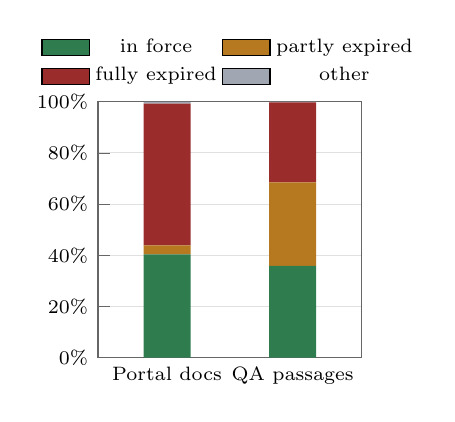
\begin{tikzpicture}
\begin{axis}[lexstyle, ybar stacked, scale only axis, width=3.35cm, height=3.25cm, bar width=17pt, ymin=0, ymax=100,
  symbolic x coords={pd,qa}, xtick=data, xticklabels={Portal docs,QA passages},
  yticklabel={\pgfmathprintnumber{\tick}\%}, enlarge x limits=0.55, area legend,
  legend style={at={(0.5,1.02)}, anchor=south, legend columns=2}, ymajorgrids]
\addplot[fill=cgreen, draw=none] coordinates {(pd,40.4) (qa,35.9)};
\addplot[fill=camber, draw=none] coordinates {(pd,3.5) (qa,32.6)};
\addplot[fill=cred, draw=none] coordinates {(pd,55.4) (qa,31.3)};
\addplot[fill=cgray, draw=none] coordinates {(pd,0.7) (qa,0.2)};
\legend{in force, partly expired, fully expired, other}
\end{axis}
\end{tikzpicture}
\end{minipage}
\vspace{-1mm}
\caption{\textbf{The same question has different correct answers over time.} \emph{Left:} the provision LexGraph-VN
answers when the question is asked at each date (real system output): the 2019 decree, the same decree as amended
in 2022, and after 2025 the 2024 decree with a ``law changed'' notice. \emph{Right:} today 55\% of the 148,282 portal documents and 31\% of the 44,408
QA passages we link to them are no longer in force.}
\label{fig:teaser}
\vspace{-2mm}
\end{figure}

% ================================================================ 1
\section{Problem statement}
\vspace{-1mm}
Given a question $q$ asked at time $t_q$, return the articles that answer it \emph{under the law in force at $t_q$} and a
cited answer that says whether the rule changed. It is hard because (i) laws change constantly and retrievers trained on
static QA data return outdated articles; (ii) validity depends on links between documents (amends, replaces, guides);
(iii) citizens say ``vượt đèn đỏ'' while the law says ``không chấp hành hiệu lệnh của đèn tín hiệu giao thông''.
\textbf{RQ1} How often are retrieved articles outdated, and how much do validity signals fix it? \textbf{RQ2} Which
relation types matter? \textbf{RQ3} Can a small self-hosted LLM cite correctly and explain changes?

% ================================================================ 2
\vspace{-1mm}
\section{Datasets}
\vspace{-1mm}
\begin{table}[H]
\centering
\caption{Data. The QA pairs supervise retrieval; the knowledge graph is mined from a public CC~BY~4.0 crawl of the
vbpl.vn portal (171,556 documents; its API is closed to robots), which we parse and mine ourselves.}
\label{tab:data}
\resizebox{\linewidth}{!}{%
\begin{tabular}{lr@{\hspace{2em}}lr}
\toprule
\multicolumn{2}{l}{\textbf{Legal QA pairs}} & \multicolumn{2}{l}{\textbf{Legal knowledge graph (web mining)}} \\
\midrule
Question--article pairs / questions & 132,424 / 119,007 & Documents / articles (\textit{Điều}) & 148,282 / 981,412 \\
Passages in the corpus & 68,663 & Typed edges (9 types) & 894,330 \\
Questions with $\geq$2 gold articles & 10.1\% & Clause-level amendments extracted & 38,344 \\
Split v2 train / val / test (no duplicate text) & 95,231 / 11,891 / 11,885 & QA passages linked to their article & 64.7\% \\
Test questions whose gold law has changed & \ResNTemporal & Successor articles added to the corpus & 116,553 chunks \\
\bottomrule
\end{tabular}}
\vspace{-2mm}
\end{table}

% ================================================================ 3
\vspace{-1mm}
\section{System design}
\vspace{-1mm}
\textbf{Requirements:} answer with the law in force at any date, cite clauses, explain changes, refuse without evidence.

\begin{figure}[H]
\centering
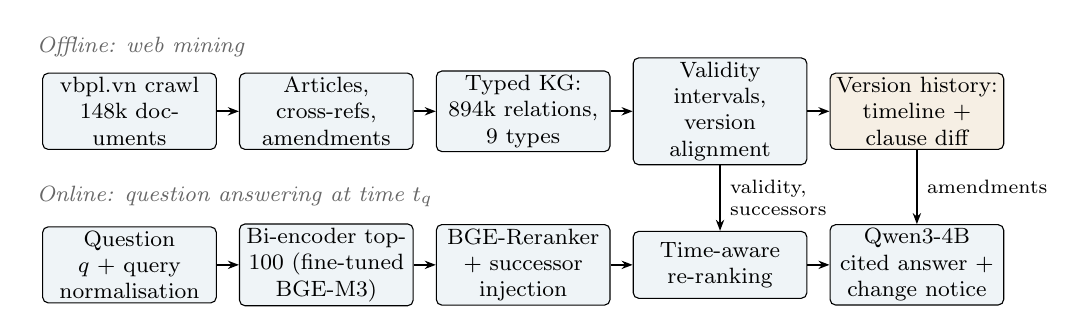
\begin{tikzpicture}[
  box/.style={draw, rounded corners=2pt, align=center, font=\footnotesize, text width=2.1cm,
              minimum height=0.85cm, inner sep=1.5pt, fill=cblue!7},
  arr/.style={-{Stealth[length=4pt]}, semithick},
  lane/.style={font=\footnotesize\itshape, anchor=west, text=black!60}]
\node[lane] at (-0.25, 0.82) {Offline: web mining};
\node[box] (crawl) at (1.05, 0)  {vbpl.vn crawl\\148k documents};
\node[box] (ie)    at (3.55, 0)  {Articles, cross-refs, amendments};
\node[box] (kg)    at (6.05, 0)  {Typed KG: 894k relations, 9 types};
\node[box] (time)  at (8.55, 0)  {Validity intervals, version alignment};
\node[box, fill=camber!12] (diff)  at (11.05, 0) {Version history: timeline + clause diff};
\node[lane] at (-0.25, -1.08) {Online: question answering at time $t_q$};
\node[box] (q)     at (1.05, -1.95)  {Question $q$ + query normalisation};
\node[box] (bi)    at (3.55, -1.95)  {Bi-encoder top-100 (fine-tuned BGE-M3)};
\node[box] (ce)    at (6.05, -1.95)  {BGE-Reranker + successor injection};
\node[box] (rr)    at (8.55, -1.95)  {Time-aware re-ranking};
\node[box] (llm)   at (11.05, -1.95) {Qwen3-4B cited answer + change notice};
\draw[arr] (crawl) -- (ie); \draw[arr] (ie) -- (kg); \draw[arr] (kg) -- (time); \draw[arr] (time) -- (diff);
\draw[arr] (q) -- (bi); \draw[arr] (bi) -- (ce); \draw[arr] (ce) -- (rr); \draw[arr] (rr) -- (llm);
\draw[arr] (time) -- node[font=\scriptsize, right, align=left] {validity,\\successors} (rr);
\draw[arr] (diff) -- node[font=\scriptsize, right] {amendments} (llm);
\end{tikzpicture}
\vspace{-1mm}
\caption{\textbf{LexGraph-VN pipeline.} \textbf{Offline}: the legal portal is mined into a knowledge graph with
typed relations, validity intervals, article versions and clause-level amendments. \textbf{Online}: articles not in force
at the question time $t_q$ move down, their newer versions move up, and Qwen3-4B answers with citations.}
\label{fig:arch}
\vspace{-2mm}
\end{figure}

\begin{wrapfigure}{r}{0.43\linewidth}
\vspace{-5mm}
\centering
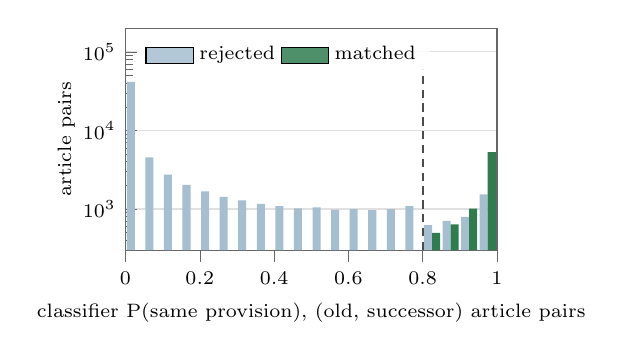
\begin{tikzpicture}
\begin{axis}[lexstyle, ybar=0pt, width=6.3cm, height=4.4cm, bar width=2.9pt, xmin=0, xmax=1.0, ymode=log, ymin=300,
  ymax=200000, xlabel={classifier P(same provision), (old, successor) article pairs}, ylabel={article pairs}, ymajorgrids,
  ylabel shift=-4pt, legend style={at={(0.03,0.97)}, anchor=north west, fill=white, fill opacity=0.85, text opacity=1,
  legend columns=2}, area legend, log origin=infty, unbounded coords=discard]
\addplot[fill=cblue!40, draw=none] coordinates {\ResAlignHistRej};
\addplot[fill=cgreen, draw=none] coordinates {\ResAlignHistAcc};
\draw[densely dashed, thick, black!70] (axis cs:\ResAlignThr,300) -- (axis cs:\ResAlignThr,60000);
\legend{rejected, matched}
\end{axis}
\end{tikzpicture}
\vspace{-2mm}
\caption{Version alignment: one-to-one matching keeps \ResAlignArtAccepted{} of \ResAlignArtPairs{} candidate pairs
(precision \ResAlignPrec{} on judged test pairs); \ResAlignAccepted{} of \ResAlignPairs{} passages get a successor.}
\label{fig:align}
\vspace{-4mm}
\end{wrapfigure}
\textbf{Knowledge graph.} We map 26 portal relation labels to 9 typed edges \emph{actor$\to$target}, checking each
direction with issue dates (the actor is newer in 96--100\% of edges per label), split the HTML into articles and extract
references with rules (P/R 0.63/0.51 against the portal's incomplete lists, plus 215,573 references it does not list).
Louvain finds 151 communities (modularity 0.58) that match legal domains.

\textbf{Temporal layer.} A passage is \emph{stale} at $t_q$ if its document is not in force, or if a document that
amends, replaces or repeals it has an article aligned with it: a gradient-boosting classifier on pair features
(similarity, cross-encoder score, overlap, relation type) trained on \ResAlignJudged{} judged pairs, then one-to-one
matching (Figure~\ref{fig:align}). Successor
articles are added to the corpus, and amending texts (``Sửa đổi điểm a khoản 3 Điều 6 như sau: \dots'') are parsed into
clause-level diffs that the demo shows as a version history.

\textbf{Re-ranking.} The bi-encoder returns the top-100 articles; the cross-encoder scores the top-30 plus the
successors of stale candidates (\emph{successor injection}); the final score is
$s(q,d) = s_{\mathrm{CE}}(q,d) - \gamma\,\mathbf{1}[d \text{ not in force at } t_q]$, with $\gamma$ tuned on validation by MRR@10 against the \emph{current} gold (a superseded gold passage is replaced by its
successor). Everyday wording is mapped to legal wording before retrieval (query normalisation).

\textbf{Fine-tuning.} Both models are trained for one epoch with DDP on 2$\times$H200. BGE-M3 uses
MultipleNegativesRankingLoss with 3 semi-hard negatives per pair, mined from the zero-shot top-100 (105,899 pairs, global
batch 128). BGE-Reranker-v2-M3 uses BCE on 1 positive and 7 negatives mined with the fine-tuned BGE-M3 (\ResCePairs{}
pairs).

\textbf{Answering.} Qwen3-4B, served with vLLM on our own GPU, receives the most relevant clauses of the articles in force,
the old version of a changed article and the amendments of the clauses shown. It must cite document, article and
clause and refuse without evidence. A ``law changed'' section is allowed only for a \emph{verified change}: the clause
asked about differs and Qwen3-4B confirms that the answer differs; other notices are removed after generation.

% ================================================================ 4
\vspace{-1mm}
\section{Current results}
\vspace{-1mm}
\pgfplotsset{panel/.style={lexstyle, scale only axis, width=3.55cm, height=2.35cm}}
\begin{figure}[H]
\centering
% ---------------- row 1
\begin{minipage}[t]{0.325\linewidth}\centering
\begin{tikzpicture}
\begin{axis}[panel, width=2.6cm, xbar, bar width=3.2pt, xmin=0.45, xmax=1.08,
  ytick=data, symbolic y coords={zs,zsce,ft,ftce}, yticklabels={BGE-M3,{+ Reranker},{BGE-M3 (FT)},{+ Reranker (FT)}},
  y dir=reverse, xmajorgrids, enlarge y limits=0.2, xtick={0.5,0.7,0.9},
  legend style={at={(0.5,1.02)}, anchor=south, legend columns=2}, area legend,
  nodes near coords, nodes near coords style={font=\tiny, anchor=west, inner sep=0.5pt}, point meta=explicit symbolic]
\addplot[fill=cblue, draw=none] coordinates {(\ResZsMrr,zs) [\ResZsMrr] (\ResZsCeMrr,zsce) [\ResZsCeMrr] (\ResFtMrr,ft) [\ResFtMrr] (\ResFtCeMrr,ftce) [\ResFtCeMrr]};
\addplot[fill=cblue!35, draw=none] coordinates {(\ResZsRten,zs) [\ResZsRten] (\ResZsCeRten,zsce) [\ResZsCeRten] (\ResFtRten,ft) [\ResFtRten] (\ResFtCeRten,ftce) [\ResFtCeRten]};
\legend{MRR@10, R@10}
\end{axis}
\end{tikzpicture}\\[-0.5mm]
{\footnotesize (a) Retrieval + re-ranking (test)}
\end{minipage}\hfill
\begin{minipage}[t]{0.325\linewidth}\centering
\begin{tikzpicture}
\begin{axis}[panel, xmin=0, xmax=1.02, ymin=0.6, ymax=0.84, xlabel={training epoch}, ylabel={val MRR@10}, ymajorgrids,
  legend style={at={(0.98,0.04)}, anchor=south east, fill=white, fill opacity=0.8, text opacity=1}, ylabel shift=-3pt]
\addplot[cblue, thick, mark=*, mark size=1.3pt] coordinates {\ResBiCurve};
\addplot[cred, thick, mark=square*, mark size=1.3pt] coordinates {\ResCeCurve};
\legend{bi-encoder, cross-encoder}
\end{axis}
\end{tikzpicture}\\[-0.5mm]
{\footnotesize (b) Fine-tuning (validation)}
\end{minipage}\hfill
\begin{minipage}[t]{0.325\linewidth}\centering
\begin{tikzpicture}
\begin{axis}[panel, width=2.9cm, xmode=log, log basis x=2, xmin=0.4, xmax=10, xtick={0.5,1,2,4,8}, xticklabels={0.5,1,2,4,8},
  xlabel={stale penalty $\gamma$}, ylabel={val MRR@10$_\text{cur}$}, ymin=0.645, ymax=0.71, ymajorgrids, ytick={0.65,0.67,0.69},
  axis y line*=left, ylabel shift=-3pt, yticklabel style={/pgf/number format/fixed, /pgf/number format/precision=2}]
\addplot[cgreen, thick, mark=*, mark size=1.3pt] coordinates {\ResGammaMrr};
\label{pl:gm}
\end{axis}
\begin{axis}[panel, width=2.9cm, xmode=log, log basis x=2, xmin=0.4, xmax=10, axis y line*=right, axis x line=none,
  ytick pos=right, yticklabel pos=right, ylabel near ticks, ylabel={Stale@10}, ymin=0, ymax=0.3, ytick={0,0.1,0.2,0.3},
  legend style={at={(0.5,1.02)}, anchor=south, legend columns=2}]
\addlegendimage{/pgfplots/refstyle=pl:gm}\addlegendentry{MRR@10$_\text{cur}$}
\addplot[camber, thick, dashed, mark=triangle*, mark size=1.5pt] coordinates {\ResGammaStale};
\addlegendentry{Stale@10}
\end{axis}
\end{tikzpicture}\\[-0.5mm]
{\footnotesize (c) Stale penalty $\gamma$ (validation)}
\end{minipage}

\vspace{0.3mm}
% ---------------- row 2
\begin{minipage}[t]{0.325\linewidth}\centering
\begin{tikzpicture}
\begin{axis}[panel, ybar, bar width=7pt, ymin=0, ymax=0.9,
  symbolic x coords={st,tt,tm}, xtick=data,
  xticklabels={{Stale@10$\downarrow$},{T-MRR$_\text{cur}$},{T-Hit@10$_\text{cur}$}},
  ymajorgrids, enlarge x limits=0.25, legend style={at={(0.5,1.02)}, anchor=south, legend columns=2}, area legend,
  nodes near coords, nodes near coords style={font=\tiny}, point meta=explicit symbolic]
\addplot[fill=cgray, draw=none] coordinates {(st,\ResStaleNoTime) [\ResStaleNoTime] (tt,\ResTmrrNoTime) [\ResTmrrNoTime] (tm,\ResThitNoTime) [\ResThitNoTime]};
\addplot[fill=cgreen, draw=none] coordinates {(st,\ResStaleTime) [\ResStaleTime] (tt,\ResTmrrTime) [\ResTmrrTime] (tm,\ResThitTime) [\ResThitTime]};
\legend{no time signals, with time signals}
\end{axis}
\end{tikzpicture}\\[-0.5mm]
{\footnotesize (d) Changed questions (test)}
\end{minipage}\hfill
\begin{minipage}[t]{0.325\linewidth}\centering
\begin{tikzpicture}
\begin{axis}[panel, ybar, bar width=5pt, ymin=0, ymax=1.05,
  symbolic x coords={before,after,both}, xtick=data, xticklabels={before,after,both},
  ylabel={Hit@10}, ymajorgrids, enlarge x limits=0.22, ylabel shift=-3pt,
  legend style={at={(0.5,1.02)}, anchor=south, legend columns=3}, area legend]
\addplot[fill=cgray, draw=none] coordinates {\ResTtSt};
\addplot[fill=cblue!45, draw=none] coordinates {\ResTtNt};
\addplot[fill=cgreen, draw=none] coordinates {\ResTtLg};
\legend{static, no time, ours}
\end{axis}
\end{tikzpicture}\\[-0.5mm]
{\footnotesize (e) Time-travel}
\end{minipage}\hfill
\begin{minipage}[t]{0.325\linewidth}\centering
\begin{tikzpicture}
\begin{axis}[panel, ybar, bar width=5pt, ymin=0, ymax=1.05,
  symbolic x coords={correct,temporal,notice,refuse}, xtick=data,
  xticklabels={correct,{changed},notice,refusal},
  ymajorgrids, enlarge x limits=0.15, legend style={at={(0.5,1.02)}, anchor=south, legend columns=3}, area legend]
\addplot[fill=cgray, draw=none] coordinates {\ResAnsNone};
\addplot[fill=cblue!45, draw=none] coordinates {\ResAnsPlain};
\addplot[fill=cgreen, draw=none] coordinates {\ResAnsOurs};
\legend{no RAG, plain RAG, ours}
\end{axis}
\end{tikzpicture}\\[-0.5mm]
{\footnotesize (f) Qwen3-4B answers}
\end{minipage}
\vspace{-1mm}
\caption{\textbf{Fine-tuning improves relevance; validity signals fix outdated answers.} (a) 11,885 test questions.
(c) Beyond $\gamma{=}2$ the penalty also hides useful context. (d) The \ResNTemporal{} test questions whose gold article
was superseded. (e) Hit@10, \ResNTt{} questions asked before and after a change. (f) \ResNAns{} answers judged by
gpt-oss-120b: correct overall / on changed questions, with a change notice, correct refusals.}
\label{fig:results}
\vspace{-2mm}
\end{figure}

\begin{table}[H]
\centering
\caption{Validity signals (fine-tuned models, test). ``cur'': gold replaced by its successor if superseded; T: changed
questions; Stale@10: share of the top 10 not in force on 23/11/2026; \ResWeights{} chosen on validation.}
\label{tab:abl}
\setlength{\tabcolsep}{5pt}
\resizebox{\linewidth}{!}{%
\begin{tabular}{lccccc}
\toprule
System & MRR@10 & MRR@10$_\text{cur}$ & Stale@10 $\downarrow$ & T-MRR@10$_\text{cur}$ & T-Hit@10$_\text{cur}$ \\
\midrule
\ResAblRows
\bottomrule
\end{tabular}}
\vspace{-2mm}
\end{table}

\textbf{Findings.}
\begin{itemize}[leftmargin=1.2em, itemsep=0pt, topsep=1pt]
\item \textbf{RQ1 (outdated answers):} without validity signals \ResStaleNoTimePct{} of the top-10 results are no longer in
force; the stale penalty and successor injection cut this to \ResStaleTimePct{} and raise MRR@10 under the current law on
changed questions from \ResTmrrNoTime{} to \ResTmrrTime. Asked before and after a change, the system is right at both dates for \ResTtBothPct{} of questions (static RAG: \ResTtStaticBothPct).
\item \textbf{RQ2 (relation types):} amends or replaces/repeals edges alone lower T-MRR@10$_\text{cur}$ to
\ResTmrrAmends/\ResTmrrRepl, so both are needed; the judge accepts \ResAlignAccPct{} of audited alignments.
\item \textbf{RQ3 (answers):} time-aware RAG raises judged correctness from \ResAnsPlainCorrect{} to \ResAnsCorrect{}
(no retrieval: \ResAnsNoneCorrectPct); notices cover \ResAnsNoticeRecallPct{} of really changed answers, with
\ResAnsFalseAlarmPct{} false notices on stable questions.
\end{itemize}

% ================================================================ 5
\vspace{-1mm}
\section{System status and next steps}
\vspace{-1mm}
\textbf{Done} (end to end on our server): knowledge graph, temporal layer, amendments, fine-tuned \mbox{BGE-M3} and
BGE-Reranker, Qwen3-4B on vLLM, demo with time-travel and version history.
\textbf{Next (final report):} incremental vbpl.vn crawling with live graph updates; higher alignment recall; old
versions as hard negatives; NLI citation checks.

\end{document}
